\chapter{Strongly Connected Directed Graphs}
Rishnak wanted to continue his discussion with Ajur on the topic of directed graphs and caught up with Ajur and jura on their stroll. Rishnak started with asking Ajur if Ajur remembered what relations are. Ajur replied that the relation could be symmetric like a facebook friend (that is if A is a friend of B, then B is also a friend of A - resulting in a friendship
undirected graph.
The relation can also be asymmetric -like a twitter follower (that is if X follows the twitter
feed of Y, Y need not follow the twitter feed of X) - resulting in a twitter directed graph.
Rishnak added that there are many relations which are asymmetric like less than or precedence relations or parent relation or winner relation. In each case, we get a directed graph representing the asymmetric relation.
Similar to path and walk in an undirected graph, we can define path and walk in directed graph (which we discussed in Chapter 6).

An undirected graph is connected if there is a path between every pair of vertices. A directed graph is strongly connected, if there is directed path between every pair of vertices. Rishnak showed the following example Figure \ref{15g1}

\begin{figure}
\begin{center}
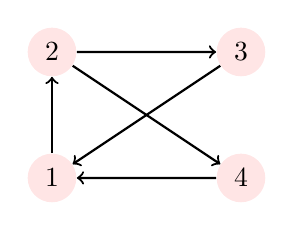
\begin{tikzpicture}
  [scale=.8,auto=left,every node/.style={circle,fill=red!10}]
  \node (n1) at (1,7) {1};
  \node (n2) at (1,9)  {2};
  \node (n3) at (4,9)  {3};
  \node (n4) at (4,7) {4};
 \path[->, draw,thick] 
        (n1) edge (n2)
         (n3) edge (n1)
        (n2) edge (n3)
        (n2) edge (n4)
        (n4) edge  (n1);

\end{tikzpicture}
\caption{ Strongly connected digraph - there is a path between every pair of vertices}\label{15g1}
\end{center}
\end{figure}

Ajur noted that the above directed graph remains strongly connected with fewer number of edges and  drew the graph in Figure \ref{15g2}

\begin{figure}
\begin{center}
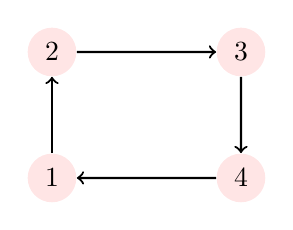
\begin{tikzpicture}
  [scale=.8,auto=left,every node/.style={circle,fill=red!10}]
  \node (n1) at (1,7) {1};
  \node (n2) at (1,9)  {2};
  \node (n3) at (4,9)  {3};
  \node (n4) at (4,7) {4};
 \path[->, draw,thick] 
         (n1) edge (n2)
        (n2) edge (n3)
        (n3) edge (n4)
        (n4) edge  (n1);

\end{tikzpicture}
\caption{ Strongly connected digraph - there is a path between every pair of vertices and has the smallest number of edges}\label{15g2}
\end{center}
\end{figure}

Pleased, Rishnak added that a strongly connected directed graph should have at least $n$ edges. But a directed graph may not be strongly connected even with $\frac{n \times (n-1)}{2}$ edges - an example is shown in Figure \ref{15g3}
\begin{figure}
\begin{center}
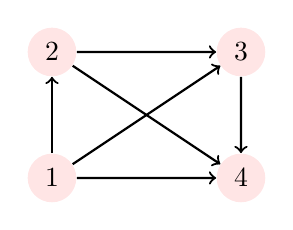
\begin{tikzpicture}
  [scale=.8,auto=left,every node/.style={circle,fill=red!10}]
  \node (n1) at (1,7) {1};
  \node (n2) at (1,9)  {2};
  \node (n3) at (4,9)  {3};
  \node (n4) at (4,7) {4};
 \path[->, draw,thick] 
        (n1) edge (n2)
         (n1) edge (n3)
        (n2) edge (n3)
        (n2) edge (n4)
        (n3) edge (n4)
        (n1) edge  (n4);

\end{tikzpicture}
\caption{ Not a strongly connected directed graph and as no vertex can reach vertex 1}\label{15g3}
\end{center}
\end{figure}

Rishnak then asked Ajur how many edges one needed to add to Figure \ref{15g3} to make it strongly connected. Ajur thought a bit and said if an edge from vertex 4 to vertex 1 is added then the digraph would become strongly connected. Rishnak was impressed with Ajur's immediate reponse. Probing further, Rishnak asked Ajur how many edges should be removed from Figure \ref{15g1} to make it not strongly connected. Ajur was up to task and answered that if edge from vertex 1 to 2 is deleted then the directed graph is not strongly connected (as no vertex is reachable from vertex 1.) \footnote{Edge deletion problems relate to edge failures and they have been well studied.}

Transitive closure of a directed graph $G=(V,E)$ is a directed graph $H=(V,E_1)$ that there is a directed edge between two vertices $x$ and $y$, if there is a directed path from vertex $x$ to vertex $y$ in $G$. Ajur could not contain his excitement and said that the transitive closure of a strongly connected graph will be a complete directed graph. Ajur gave the following reasons of his observation:
\begin{enumerate}
    \item In the orginal directed graph there is a directed path between very pair of vertices as it is given to be strongly connected.
    \item In the transitive closure graph there is an edge between every pair of vertices as there is a path between every pair of vertices in the original graph.
\end{enumerate}

For example, here is the transitive closure of directed graphs shown in Figures \ref{15g1} and \ref{15g2} is given in Figure \ref{15g4}

\begin{figure}
\begin{center}
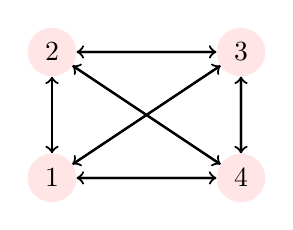
\begin{tikzpicture}
  [scale=.8,auto=left,every node/.style={circle,fill=red!10}]
  \node (n1) at (1,7) {1};
  \node (n2) at (1,9)  {2};
  \node (n3) at (4,9)  {3};
  \node (n4) at (4,7) {4};
 \path[->, draw,thick] 
         (n1) edge (n2)
         (n2) edge (n1)
        (n2) edge (n3)
        (n3) edge (n2)
        (n3) edge (n4)
        (n4) edge (n3)
        (n1) edge (n4)
        (n1) edge (n3)
        (n3) edge (n1)
        (n2) edge (n4)
        (n4) edge (n2)
        (n4) edge  (n1);

\end{tikzpicture}
\caption{ Transitive closure of graphs in \ref{14g1} and \ref{14g2}}\label{15g4}
\end{center}
\end{figure}

For example in a facebook page or a twitter feed, if some one posts a message, it will be visible to his friends. If his friends share that post or tweet, then that post will be visible to all the friends of that friend. That is how transitive closure works. If you post any message in a social media, it will be seen
by almost every one!


Rishnak then told Ajur about the book "Dudney 536 Puzzles and Curious Problems" and that one particular problem in that book may be of interest to Ajur and relevant to this topic. Problem number 452 says that there are four teams Scotland, England, Wales and Ireland. The following table \ref {14t1} shows the result of their matches. Rishnak asked Ajur can he draw a directed graph for this? 
\begin{table}
\begin{center}
\begin{tabular}{ |p{3cm}||p{1.5cm}||p{1.5cm}||p{1.5cm}||p{1.5cm}||  }
 \hline
 \multicolumn{5}{|c|}{Result of Games} \\
 \hline
 Country Name & Played &Won&Lost&Drawn\\
 \hline
 Scotland  & 3    &3&0&0\\
 England& 3& 1 &1&1\\
 Wales&3 &1&1&1\\
 Ireland    &3 &0&3&0\\
 
 \hline
\end{tabular}
\caption{Results of 6 Soccer Matches}\label{14t1}
\end{center}
\end{table}

Ajur thought for a bit and he was able to draw the directed graph as Scotland won all matches and Ireland lost all matches and hence Wales and England must have drawn. His directed graph is shown in Figure \ref{15g33}.

\begin{figure}
\begin{center}
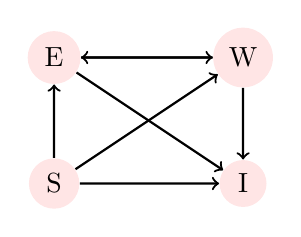
\begin{tikzpicture}
  [scale=.8,auto=left,every node/.style={circle,fill=red!10}]
  \node (n1) at (1,7) {S};
  \node (n2) at (1,9)  {E};
  \node (n3) at (4,9)  {W};
  \node (n4) at (4,7) {I};
 \path[->, draw,thick] 
         (n1) edge (n2)
         (n1) edge (n3)
         (n1) edge (n4)
        (n2) edge (n4)
        (n2) edge (n3)
        (n3) edge (n2)
        (n3) edge (n4);

\end{tikzpicture}
\caption{ A Directed Graph for Soccer Matches, S represents Scotland, E represents England, W represents Wales and I represents Ireland}\label{15g33}
\end{center}
\end{figure}

Rishnak added that Scotland defeated England by 3-0 and the rest of the goals for and against as
shown below \ref{14t2} Rishank asked Ajur whether he can get all the scores of the rest of the 5 games.
\begin{table}
\begin{center}
\begin{tabular}{ |p{3cm}||p{1.5cm}||p{1.5cm} || }
 \hline
 \multicolumn{3}{|c|}{Goals} \\
 \hline
 Country Name & For&Against\\
 \hline
 Scotland  & 7    &1\\
 England& 2&3\\
 Wales&3&3\\
 Ireland&1&6\\
 
 \hline
\end{tabular}
\caption{Goals For and Against}\label{14t2}
\end{center}
\end{table}

Ajur was challenged. He could get the scores of England immediately, England defeated Ireland by a score of 2-0 and drew with Wales 0-0. Now he reasoned Scotland defeated Wales by a score of 2-1 and defeated Ireland by a score 2-0.\footnote{Ajur tried various combinations and failed and finally got this.} These
satisfied the goals for and Against Scotland and England. Finally Wales defeated Ireland by a score of 2-1
and all things matched.
Ajur drew the following table \ref{14t3}

\begin{table}
\begin{center}
\begin{tabular}{ |p{3cm}||p{3cm}||p{1.5cm} || }
 \hline
 \multicolumn{3}{|c|}{Game Scores} \\
 \hline
 Country Name & Country Name &Score\\
 \hline
 Scotland  & England    &3-0\\
 Scotland& Wales&2-1\\
 Scotland&Ireland&2-0\\
 England&Wales&0-0\\
 England&Ireland &2-0\\
 Wales&Ireland&2-1\\
 
 
 \hline
\end{tabular}
\caption{Goal Scores in Six Soccer Games}\label{14t3}
\end{center}
\end{table}
A directed graph is acyclic (sometimes called as Directed Acyclic Graph or DAG), if there are no directed cycles in the graph. Ajur drew an example of a DAG in Fifure \ref{15g5}

\begin{figure}
\begin{center}
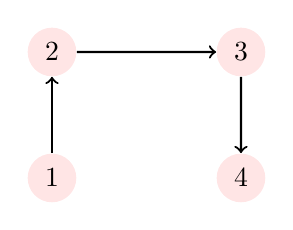
\begin{tikzpicture}
  [scale=.8,auto=left,every node/.style={circle,fill=red!10}]
  \node (n1) at (1,7) {1};
  \node (n2) at (1,9)  {2};
  \node (n3) at (4,9)  {3};
  \node (n4) at (4,7) {4};
 \path[->, draw,thick] 
         (n1) edge (n2)
        (n2) edge (n3)
        (n3) edge (n4);

\end{tikzpicture}
\caption{ A Directed Acyclic Graph}\label{15g5}
\end{center}
\end{figure}

Rishnak said that DAG may also contain an undirected cycle but not a directed cycle and hence it is still called a DAG. Rishnak added a few more edge to Figure \ref{15g5} and still remained acyclic as shown in Figure \ref{15g6}

\begin{figure}
\begin{center}
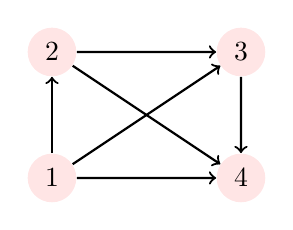
\begin{tikzpicture}
  [scale=.8,auto=left,every node/.style={circle,fill=red!10}]
  \node (n1) at (1,7) {1};
  \node (n2) at (1,9)  {2};
  \node (n3) at (4,9)  {3};
  \node (n4) at (4,7) {4};
 \path[->, draw,thick] 
         (n1) edge (n2)
        (n2) edge (n3)
        (n1) edge (n3)
        (n3) edge (n4)
        (n1) edge (n4)
        (n2) edge (n4);

\end{tikzpicture}
\caption{ A Directed Acyclic Graph - even though it contains undirected cycles }\label{15g6}
\end{center}
\end{figure}

\textbf{Question for thirteenth day:} Rishnak asked Ajur how he would make the digraph in Figure \ref{15g5} strongly connected. 

\textbf{Answer:} Ajur responded immediately saying  addition of a directed edge from vertex 4 to vertex 1 would make that digraph strongly connected.

It was getting dark and Jura and Ajur wanted to continue on their stroll. Rishnak bade them good night.
